\documentclass[11pt,a4paper]{article}
\usepackage[T1]{fontenc}
\usepackage{lmodern,microtype,amsmath,amssymb,mathtools}
\usepackage[a4paper,margin=22mm,headheight=15pt,headsep=7mm,footskip=11mm]{geometry}
\usepackage{graphicx,booktabs,array,longtable,xcolor}
\usepackage{titlesec,fancyhdr,enumitem,xurl,needspace}
\usepackage[hidelinks,pdfauthor={Sai Reddivari}]{hyperref}
\definecolor{ink}{HTML}{183B48}
\definecolor{muted}{HTML}{56656D}
\definecolor{teal}{HTML}{247B82}
\setlength{\parindent}{0pt}\setlength{\parskip}{6pt plus 1pt}
\setlength{\emergencystretch}{2em}\renewcommand{\arraystretch}{1.18}
\setlist{nosep,leftmargin=1.4em}\setcounter{secnumdepth}{0}
\titleformat{\section}{\Large\bfseries\color{ink}}{}{0pt}{}
\titleformat{\subsection}{\large\bfseries\color{ink}}{}{0pt}{}
\titleformat{\subsubsection}{\normalsize\bfseries}{}{0pt}{}
\titlespacing*{\section}{0pt}{10pt}{8pt}\titlespacing*{\subsection}{0pt}{10pt}{5pt}
\pagestyle{fancy}\fancyhf{}
\fancyhead[L]{\small\color{muted}Economic features and selection risk in USD/JPY}
\fancyhead[R]{\small\color{muted}Sai Reddivari}
\fancyfoot[L]{\footnotesize\color{muted}Research study \enspace | \enspace October 2026}
\fancyfoot[R]{\small\thepage}\renewcommand{\headrulewidth}{.3pt}
\widowpenalty=10000\clubpenalty=10000
\newcommand{\captiontext}[1]{{\small\color{muted}#1\par}}
\newcommand{\nextpage}{\clearpage}

\hypersetup{pdftitle={Economic features and selection risk in daily USD/JPY forecasting}}
\begin{document}
\thispagestyle{plain}
{\small\sffamily\color{muted}RESEARCH STUDY \hfill 29 OCTOBER 2026}\par
\vspace{10pt}
{\fontsize{25}{29}\selectfont\bfseries\color{ink}Economic features and selection risk in daily USD/JPY forecasting\par}
\vspace{8pt}{\normalsize Sai Reddivari}\par
{\small\color{muted}An availability-aware comparison of three boosting models and simpler baselines}\par
\vspace{5pt}{\color{teal}\hrule height .8pt}\vspace{8pt}

\textbf{Abstract.} Can economically motivated information improve prediction of a meaningful positive USD/JPY move beyond the currency's own recent history? This study constructs 39 candidate features spanning relative rates, Japanese equity sectors, global risk, dollar strength, commodities and positioning. Three selection designs are compared over eight chronological development quarters. A larger backward-search budget produced substantial inner-validation gains that failed to generalize. A controlled replay without that wrapper improved LightGBM and CatBoost, while XGBoost changed little. The resulting procedure was frozen before evaluation on 229 eligible decisions in a historical reserved year. Expanded-input XGBoost achieved mean quarterly ROC-AUC of 0.617 versus 0.553 for its own-price counterpart and 0.549 for own-price logistic regression. CatBoost reached 0.597; LightGBM did not improve on its own-price comparator. These are conditional ranking results, qualified by historical hindsight, timing assumptions, selective coverage and weak precision. They do not establish a trading edge.

\section*{The contribution is a test of the research process as well as the predictors}
USD/JPY offers several plausible channels through which external information could matter: policy divergence changes the incentive to hold dollars; yen-funded positions can unwind under stress; Japanese bank and exporter returns may reflect different domestic expectations. The aim was to turn these mechanisms into measurable, time-aligned hypotheses, then test their incremental value. Economic diversity was a reason to investigate the features, not a claim that they were independent or predictive.

The most informative result came from interrogating selection itself. Chronological validation protects an individual fit from future outcomes, but repeated subset comparisons can still adapt to noise in the same validation quarters. Here, expanding the search improved the scores used to choose subsets without improving subsequent prediction. Keeping a broader screened shortlist was more useful than continuing to optimize that search.

The implementation makes the decisions inspectable: native-calendar transformations precede as-of alignment; observation age is distinct from publication age; label intervals are purged at evaluation boundaries; frozen configurations and thresholds are recorded; and the refactored Python pipeline was compared with saved research artifacts. The public package exposes this logic and aggregate evidence while marking the private inputs needed for full reproduction.

\vfill
\captiontext{Reading guide. Pages 2--4 define the information set, all candidate features and evaluation. Pages 5--6 explain the selection experiments. Pages 7--8 report the original reserved evaluation and a separate post-hoc sensitivity. Pages 9--10 cover implementation, limitations and next decisions. The optional appendix supplies implementation details, grids and expanded tables.}

\nextpage
\section*{Economic hypotheses become features only after their clocks are aligned}
Collection covers 22 October 2020--21 October 2025 for development and a reserved year ending 21 October 2026. Rolling warm-ups leave a feature-complete development start of 19 November 2021. The pool includes the currency's own state: external inputs must improve on a credible price-history baseline, not merely a constant forecast.

The candidate table on the next page makes the hypotheses explicit. Relative rates describe policy divergence; Japanese sectors add domestic-market information; US equities, volatility and commodities describe the environment in which yen-funded risk may unwind. Positioning adds a separate view of exposure and fragility. The currency's own returns and volatility provide the baseline against which these external inputs must earn their place.

Transformations precede alignment on native calendars: five Tokyo sessions are not five US sessions, and 52 distinct reports are not 260 repeated daily observations. Returns and changes reduce dependence on arbitrary levels; they do not guarantee stationarity. Three declared derived contrasts/products are part of the 39-column pool, rather than a search over every possible interaction.

\begin{center}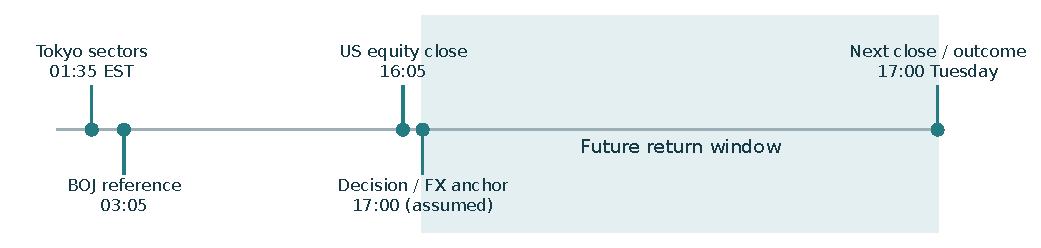
\includegraphics[width=\linewidth]{../figures/information_clock.pdf}\end{center}
\captiontext{Figure 1. Ordinary winter-session illustration. Markers are adopted availability times, not a verified vendor-delivery log. The label starts at the decision cutoff; an input published during that future interval is unavailable to the decision.}

The FMP daily FX close is provisionally assigned to 17:00 New York, including the target and dollar basket. Equity closes have a five-minute visibility buffer. Tokyo clocks use time-zone conversion. Japanese market observations use market-visibility assumptions rather than simply their later government publication times. These conventions do not prove historical point-in-time access. The appendix lists source-specific qualifications.

\subsection*{How to read the feature definitions}
Write $\ell_k(A)_d=\log(A_d/A_{d-k})$ for a log return and $\Delta_k x_d=x_d-x_{d-k}$ for a change. $r_t=P_t/P_{t-1}-1$ is the simple FX return; $s_k$ is sample standard deviation and $\overline P_k$ a trailing price mean. Trailing standardization is $z_n(x)=(x-\overline x_n)/s_n(x)$, including the current available value. Horizons use native source sessions before alignment, except rate-gap changes and 260-row z-scores, which use decision rows. Positioning uses distinct reports. These conventions apply throughout the candidate table.

\nextpage
\section*{The feature set translates economic hypotheses into measurable inputs}
\label{sec:feature-map}
All 39 candidates are listed below; multiple horizons count as separate columns. A dagger ($\dagger$) marks the five removed in the final fit; the other 34 entered all three frozen expanded-input boosters. Retention is not evidence of individual predictive value.

\begingroup\small
\setlength{\tabcolsep}{4pt}\renewcommand{\arraystretch}{1.09}
\begin{tabular}{@{}>{\raggedright\arraybackslash}p{.225\linewidth}>{\raggedright\arraybackslash}p{.445\linewidth}>{\raggedright\arraybackslash}p{.285\linewidth}@{}}
\toprule
Feature family and inputs & Definition & Economic intuition to test\\\midrule
\textbf{Currency state (10)}\newline
Returns: $1^\dagger,5,20^\dagger$\newline
Absolute daily return\newline
20-session volatility\newline
Volatility ratio$^\dagger$\newline
MA distance: $20^\dagger,60$\newline
Tokyo reference to close\newline
Weekend flag
& \mbox{}\newline $\ell_k(P)$, $k\in\{1,5,20\}$\newline
$|\ell_1(P)|$\newline
$v_t=s_{20}(r)_t$\newline
$s_5(r)_t/s_{20}(r)_t$\newline
$P_t/\overline P_{k,t}-1$, $k\in\{20,60\}$\newline
$P_t/\mathrm{BOJfix}_{\mathrm{latest}}-1$\newline
$\mathbf1\{(t,t+1]\text{ spans a weekend}\}$
& Trend/reversal, volatility and price stretch; Europe-inclusive reference-to-close movement and weekend exposure. The own-price baseline.\\[4pt]
\textbf{Relative rates (5)}\newline
Two-year gap\newline
Gap change: 1, 5\newline
US slope change$^\dagger$\newline
Japan slope change
& \mbox{}\newline $g_t=US2y_{\mathrm{latest}}-JP2y_{\mathrm{latest}}$\newline
$\Delta_k g_t$, $k\in\{1,5\}$\newline
$\Delta_5(US10y-US2y)$\newline
$\Delta_5(JP10y-JP2y)$
& Carry and policy repricing; curve shape adds growth context. Eligible yield legs may have different observation dates.\\[4pt]
\textbf{Japanese sectors (4)}\newline
Banks relative: 5, 20\newline
Electronics relative: 5\newline
TOPIX: 5
& \mbox{}\newline $\ell_k(Banks)-\ell_k(TOPIX)$, $k=5,20$\newline
$\ell_5(Electronics)-\ell_5(TOPIX)$\newline
$\ell_5(TOPIX)$
& Domestic-rate sensitivity and Japanese equity conditions. Electronics includes precision instruments, not only exporters.\\[4pt]
\textbf{Global risk (8)}\newline
VIX level; changes: 1, 5\newline
SPY returns: 1, 5\newline
QQQ relative: 5, 20\newline
SMH relative: 5
& \mbox{}\newline $VIX$; $\Delta_k VIX$, $k=1,5$\newline
$\ell_k(SPY)$, $k=1,5$\newline
$\ell_k(QQQ)-\ell_k(SPY)$, $k=5,20$\newline
$\ell_5(SMH)-\ell_5(QQQ)$
& Risk repricing and potential carry unwinds; distinguish technology/semiconductor leadership from broad market moves.\\[4pt]
\textbf{Dollar / yen (2)}\newline
Ex-yen dollar basket: 5\newline
Yen-relative move: 5
& \mbox{}\newline $B_5=\tfrac15[-\ell_5(EURUSD)-\ell_5(GBPUSD)$\newline
$\phantom{B_5=} -\ell_5(AUDUSD)+\ell_5(USDCAD)$\newline
$\phantom{B_5=} +\ell_5(USDCHF)]$\newline
$\ell_5(P)-B_5$
& Dollar-wide versus relative yen moves. Equal weights/unit exposure are assumptions, not identification of a pure yen shock.\\[4pt]
\textbf{Commodities (2)}\newline
Lagged WTI return: 5\newline
Gold return: 5
& \mbox{}\newline $\ell_5(WTI)_{d-1}$\newline
$\ell_5(GLD)_d$
& Energy-import and monetary/risk context. Oil uses the previous native observation.\\[4pt]
\textbf{Positioning (6)}\newline
Net yen / open interest\newline
Change: 4 reports\newline
Published-report age\newline
Positioning z-score\newline
Volatility z-score\newline
Short-yen stress
& \mbox{}\newline $q_j=(LF\ longs_j-LF\ shorts_j)/OI_j$\newline
$q_j-q_{j-4}$\newline
$\operatorname{round}(\text{hours since release},3)/24$\newline
$z_{52\,\mathrm{reports}}(q)_j$\newline
$z_{260}(v)_t$\newline
$\max(0,-q_j)\max(0,z_{260}(v)_t)$
& Crowding, adjustment and information age. Positive $q$ means long yen. Stress combines short exposure and high volatility, not total carry leverage.\\[4pt]
\textbf{Scheduled events (1)}
& $\mathbf1\{\text{known scheduled event in }(t,t+1]\}$
& FOMC, BOJ, US CPI or payrolls: news exposure, not the outcome.\\[4pt]
\textbf{Rate--risk interaction (1)}
& $z_{260}(\Delta_5g)_t\,z_{260}(\Delta_5VIX)_t$
& Distinguish rate repricing in calm and stressed conditions.\\\bottomrule
\end{tabular}
\endgroup
\vspace{4pt}
\captiontext{Table 1. All 39 candidates; $\dagger$ denotes exclusion from the final 34. Notation is defined on the preceding page. Exact identifiers and implementation guards remain in the appendix.}

\nextpage
\section*{The target and validation answer a narrow forecasting question}
Let $P_t$ be the retained USD/JPY close and $t+1$ the next retained session. A positive return means dollar strength against the yen. The model estimates whether the next simple return exceeds a positive, volatility-scaled hurdle:
\[
r_{t+1}=P_{t+1}/P_t-1,\qquad
h_t=\max\{0.001,\;0.5\widehat\sigma_{20,t}\},\qquad
Y_t=\mathbf1\{r_{t+1}>h_t\}.
\]
$\widehat\sigma_{20,t}$ is the sample standard deviation of the last 20 simple returns, ending at $t$. Class 0 includes small positive returns as well as flat or falling prices. No near-zero observations are deleted. This is hurdle-exceedance prediction, not a symmetric direction forecast: volatility information may predict an exceedance without predicting the sign of the conditional mean return.

\subsection*{Eight expanding development evaluations precede a frozen procedure}
Eight outer quarters run from 22 October 2023 to 21 October 2025, with 517 evaluated rows in total. Each uses eligible earlier history and three expanding chronological inner validation quarters. No outer-quarter outcomes fit that quarter's model. At both inner and outer boundaries, a training observation is purged unless
\[
\text{outcome time}_i < \min_{j\in\mathrm{validation}}\text{decision time}_j.
\]
Selection, scaling, configuration choice, early stopping and threshold choice occur within the outer training window. Inner scores are search criteria, not independent performance estimates. Once outer development results inform an amendment, those quarters also become part of research selection.

The final fit contains 1,009 rows, with decisions from 19 November 2021 to 8 October 2025 and a last outcome on 9 October. The nominal development boundary remains 21 October: nine late-development event-timing-flagged rows were excluded. Final inner validation blocks contain 64, 65 and 56 rows. Each procedure is refitted once and frozen for the reserved year, without quarterly updates.

\subsection*{Ranking, classification and comparators are separate choices}
The primary metric is equally weighted mean quarterly ROC-AUC. Pooled AUC is secondary. Paired differences use identical rows within each quarter before averaging:
\[
\overline A_m=\frac1K\sum_{q=1}^K A_{m,q},\qquad
\Delta_{m,b}=\frac1K\sum_{q=1}^K(A_{m,q}-A_{b,q}).
\]
This prevents a large quarter from dominating the primary score, but gives small quarters equal weight. Quarter SD is dispersion, not a standard error or significance test. Four dependent quarterly comparisons cannot establish a persistent advantage.

Each booster is compared with its own-price version under the same tuning rules and with L2 logistic regression on ten currency-state inputs. A constant training-prevalence score supplies a within-quarter AUC floor of 0.5. Binary thresholds maximize balanced accuracy on pooled inner predictions and remain fixed downstream. AUC does not select a trading rule; classification is reported separately.

The reserved period is untouched by fitting and tuning, but some hypotheses were informed by commentary about that historical period. It is a reserved model evaluation, not a fully prospective test of the entire research process.

\nextpage
\section*{A larger search budget exposed selection optimism}
The initial funnel had four stages. A label-free screen removed constants, duplicates and near-duplicates using complete-linkage clustering of absolute Spearman correlations at 0.90. A light mutual-information screen removed persistently weak marginal candidates while protecting family representation and declared interaction components. Elastic-net logistic regression and grouped LightGBM permutation importance supplied complementary routes; their union formed a shortlist. Finally, a backward wrapper tested individual and grouped removals against the same three inner validation quarters.

\subsection*{Run A: the intended pruning search was budget-constrained}
The wrapper used an early-stopped LightGBM scorer and a 400-fit budget per outer fold. With 34 candidates and three inner folds, testing the first individual removals alone costs about 102 fits. The pilot also selected very short ensembles: its first-fold median was three trees. Capacity and budget concerns were identified before the complete A results returned; short ensembles alone do not prove underfitting.

Across eight folds the budget ran out after three to nine backward steps, retaining 9--33 features. Booster mean AUCs were 0.534, 0.531 and 0.547 for LightGBM, XGBoost and CatBoost, all below own-price logistic at 0.556. This tested a constrained search, not a decisive rejection of the candidate features.

\subsection*{Run B: substantial inner gains did not transfer to the next quarter}
The selection scorer changed to a fixed 150 trees at learning rate 0.03 and the wrapper budget increased to 2,000 fits. No fold exhausted it. Shortlists of 24--35 columns became subsets of 3--16; selected subsets improved inner AUC by approximately 0.07--0.21 relative to their starting shortlists.

Subsequent-quarter performance nevertheless deteriorated for LightGBM and CatBoost. Chronological splitting did not prevent search from adapting to repeatedly consulted inner outcomes. B also expanded final grids from eight to sixteen configurations and added matched own-price boosters, so A versus B alone does not isolate the wrapper's effect.

\begin{center}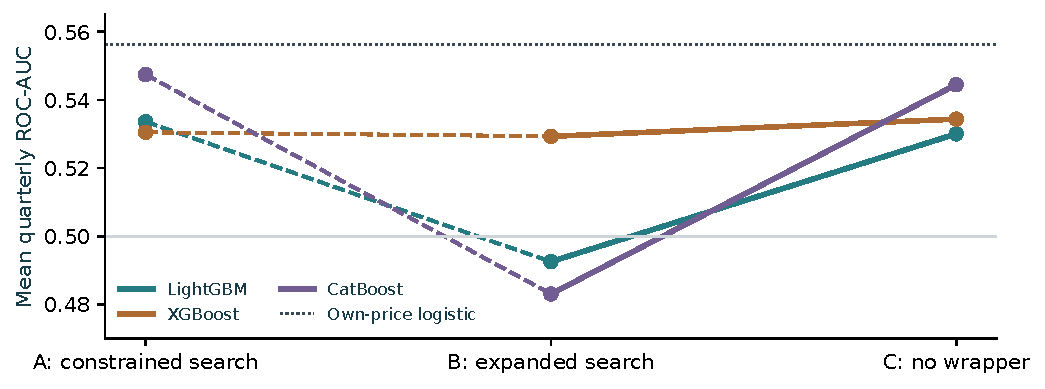
\includegraphics[width=.95\linewidth]{../figures/selection_comparison.pdf}\end{center}
\captiontext{Figure 2. Mean AUC on the same eight development quarters. A to B changes multiple settings (dashed segments); B to C removes the wrapper while holding upstream selection and downstream tuning rules fixed (solid segments). None beats the unchanged logistic baseline. Saved results; no new fits.}

\nextpage
\section*{A controlled replay supported removing the wrapper}
Run C retained B's upstream stages, feature definitions, evaluation rows and sixteen-configuration grids, but passed each complete shortlist to the final models. Each booster was retuned under the same rules for the changed inputs. This isolates removal of the wrapper more closely than A/B; it does not hold the fitted models themselves fixed.

\begin{center}\small
\begin{tabular}{@{}lrrrrrr@{}}\toprule
Model & A & B & C & $C-B$ & C wins & Own price\\\midrule
LightGBM & 0.534 & 0.493 & 0.530 & +0.037 & 6/8 & 0.530\\
XGBoost & 0.531 & 0.529 & 0.534 & +0.005 & 4/8 & 0.507\\
CatBoost & 0.547 & 0.483 & 0.544 & +0.061 & 6/8 & 0.493\\
\bottomrule\end{tabular}\end{center}

\captiontext{Table 2. Eight-quarter development means. Positive-quarter counts pair C with B on identical dates. Own-price boosters use matched sixteen-configuration grids; logistic remains 0.556. XGBoost's 0.005 change is small, not a material discovery.}

The no-wrapper replay improved LightGBM and CatBoost in six of eight quarters, but produced no development winner over logistic. The defensible decision was to simplify a component whose search had not earned its complexity, not claim that backward selection is generally ineffective.

\subsection*{Negative controls diagnose search; they do not certify an edge}
Twenty circular label shifts disrupted the original feature--outcome alignment. The matched reduced B chain scored 0.521 on real labels; shifted runs ranged from 0.454 to 0.537, with two at least as high. Its mean inner wrapper gain was 0.114, versus 0.123 across shifted runs; eleven of twenty shifted gains reached or exceeded it. Large apparent improvements were attainable without the original alignment.

The separate own-price logistic control scored 0.556 on real labels, with one of twenty shifted runs at least as high. These are descriptive falsification checks, not formal significance tests: circular shifts preserve some dependence and can alter regime alignment. The reduced B control is not a null distribution for the tuned final boosters. Matched full-procedure controls were not run for A, C or the reserved evaluation.

\subsection*{The final freeze remained development-informed}
The rule written before C's replay selected the higher-mean procedure between B and C for each booster; all selected no-wrapper. CatBoost was nominated on development mean AUC of 0.5445, versus 0.5344 for XGBoost and 0.5300 for LightGBM. This lock followed amendments; it was not registered before all research began.

On the full final training window the selection counts were
\[
39\xrightarrow{\text{structural screen}}39
\xrightarrow{\text{light MI}}34
\xrightarrow{\text{selector union}}34.
\]
Only MI removed columns in that fit. Retention does not establish that every survivor was useful. All three expanded-input boosters received the same 34 features. The final elastic-net solver was seeded at zero; development versions were unseeded and were not retrospectively rerun to manufacture reproducibility.

\nextpage
\section*{XGBoost led the reserved ranking; the advantage was not uniform}
The reserved year has 258 labelled decisions from 22 October 2025 through 20 October 2026, with outcomes through 21 October. The locked CFTC observation-age rule excluded 29 dates from the common primary scoring sample. The original evaluation therefore has 229 decisions and 64 positives, with quarter sizes of 35, 64, 65 and 65. Models and thresholds stayed frozen.

\begin{center}\small
\begin{tabular}{@{}lrrrrrr@{}}\toprule
Procedure & R1 & R2 & R3 & R4 & Mean & Pooled\\\midrule
XGBoost: shortlist & 0.630 & 0.657 & 0.639 & 0.542 & 0.617 & 0.615\\
CatBoost: shortlist & 0.606 & 0.645 & 0.677 & 0.460 & 0.597 & 0.593\\
LightGBM: shortlist & 0.576 & 0.632 & 0.543 & 0.356 & 0.527 & 0.521\\
Logistic: own price & 0.458 & 0.564 & 0.685 & 0.488 & 0.549 & 0.566\\
XGBoost: own price & 0.583 & 0.610 & 0.583 & 0.434 & 0.553 & 0.552\\
CatBoost: own price & 0.475 & 0.470 & 0.666 & 0.411 & 0.505 & 0.520\\
LightGBM: own price & 0.502 & 0.629 & 0.594 & 0.442 & 0.542 & 0.532\\
\bottomrule\end{tabular}\end{center}

\captiontext{Table 3. Original 229-row evaluation. Mean is the primary equal-quarter AUC; pooled ranks all predictions together. The constant-prevalence baseline is 0.500 for both. R1 contains only eight positives. Full dispersion and classification tables appear in the appendix.}

Expanded XGBoost exceeded its own-price twin in every quarter: mean paired gain 0.064. Its gain over logistic was 0.068, positive in three quarters. CatBoost exceeded its twin by 0.092 on the mean, subject to the qualification below. LightGBM's own-price comparison was $-0.015$.

\begin{center}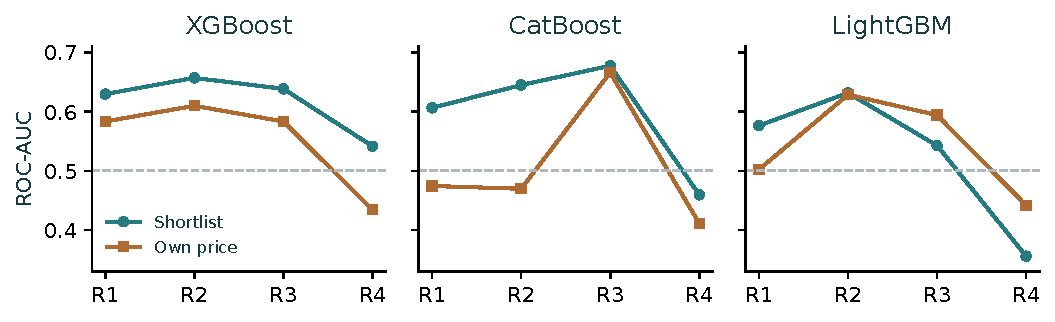
\includegraphics[width=\linewidth]{../figures/reserved_pairs.pdf}\end{center}
\captiontext{Figure 3. Shortlist versus own-price on identical reserved dates. Horizontal reference: AUC 0.5. All nonconstant models weakened from R3 to R4. Different panels are not independent experiments.}

Own-price CatBoost used five trees and classified 228 of 229 rows positive at its frozen threshold. Its effective leaf-estimation default was one Newton step versus ten for the expanded model. Matched grids therefore did not produce a strict features-only intervention. Against logistic, CatBoost gained 0.048 in mean AUC in only two quarters. Narrow probabilities do not invalidate AUC, but weak comparators and differing defaults limit attribution.

CatBoost remains the development nominee; XGBoost won the reserved ranking. This prioritizes XGBoost for a new test, not a retroactive declaration that it was the prospectively selected winner. SHAP can describe which inputs the fitted models used, not which mechanism caused successful forecasting.

\nextpage
\section*{Coverage and operating thresholds change the interpretation}
\subsection*{Useful ranking is not the same as a useful trading signal}
The original sample's positive rate was 0.279. At fixed inner-chosen thresholds, XGBoost and CatBoost recovered many positives but generated substantially more false positives than true positives. Their mean probabilities also exceeded the observed positive rate. Ranking, calibration and the decision policy need separate evaluation.

\begin{center}\small
\begin{tabular}{@{}lrrrrr@{}}\toprule
Frozen shortlist & TP & FP & Precision & Recall & Mean probability\\\midrule
XGBoost & 41 & 85 & 0.325 & 0.641 & 0.366\\
CatBoost & 48 & 106 & 0.312 & 0.750 & 0.355\\
LightGBM & 34 & 77 & 0.306 & 0.531 & 0.336\\\bottomrule
\end{tabular}\end{center}
\captiontext{Table 4. Original 229 decisions; 64 positives. Classification operating points are not trade counts or returns. No spread, slippage, financing, sizing or execution simulation is included.}

\subsection*{The 29 missing scores came from a policy, not missing FX prices}
The pipeline marked positioning more than 35 days old as missing, measured from observation rather than publication. The publication interruption excluded 29 decisions from 29 October to 8 December 2025, all in R1. A newly released backlog report could still be too old. Every daily FX price and label existed; common feature completeness reduced scoring coverage to 229/258, or 88.8\%.

After the original results, a separate sensitivity carried the latest actually published CFTC report without the cutoff. It preserved publication order, models, thresholds, formulas and the original 229-row overlap. The oldest carried observation was about 56 days old: availability did not make it fresh. All 258 decisions were restored, with 75 positives.

\begin{center}\small
\begin{tabular}{@{}lrrrr@{}}\toprule
Model & 229: expanded & 229: own & 258: expanded & 258: own\\\midrule
XGBoost & 0.617 & 0.553 & 0.612 & 0.557\\
CatBoost & 0.597 & 0.505 & 0.593 & 0.533\\
LightGBM & 0.527 & 0.542 & 0.515 & 0.558\\
\bottomrule\end{tabular}\end{center}

\captiontext{Table 5. Mean quarterly AUC under two eligibility policies. Each input comparison uses identical dates. The 258-row analysis is post-hoc, changing inputs only on previously excluded dates; it is not another untouched test.}

The expanded XGBoost and CatBoost mean advantages survived the change but narrowed. On the 29 restored dates alone, own-price CatBoost ranked better than expanded CatBoost. Neither the small movement in annual means nor the complete FX series makes exclusion immaterial. An outage policy should be fixed prospectively, with score availability and information age evaluated alongside predictive quality.

\nextpage
\section*{Implementation turns modelling choices into inspectable contracts}
The Python implementation separates parsing, alignment, target construction, native-calendar features, splits, selection, models and evaluation. This makes a data-policy change inspectable without silently changing a model, and permits refactoring without treating a fresh fit as equivalent to a historical result.

\begingroup\small
\begin{tabular}{@{}>{\raggedright\arraybackslash}p{.25\linewidth}>{\raggedright\arraybackslash}p{.70\linewidth}@{}}\toprule
Contract & Concrete implementation and evidence\\\midrule
Inputs have provenance & Cache hashes, source routes and availability bases are recorded. Private Japanese-sector values remain outside the public package.\\
Time determines eligibility & As-of joins retain observation and availability times; source calendars, clock changes and delayed CFTC releases have explicit checks.\\
Boundaries are testable & Purge assertions compare outcome endpoints with validation cutoffs; row order, labels and masks were compared with the original pipeline.\\
Frozen means fixed & Feature order, model hashes, tree counts and thresholds identify the procedures. Original probabilities and classes were reproduced locally from saved models.\\
Missing inputs cannot silently change the task & Private-input absence raises an error rather than substituting public-only features. Output guards protect references; fitting requires explicit opt-in.\\
Publication is not full reproduction & Public aggregates rebuild the exhibits. Raw caches, model binaries and the historical archive are excluded and documented.\\\bottomrule
\end{tabular}\endgroup

The prior refactor acceptance recorded 63 passing checks in the complete local environment: data/split/configuration equivalence, frozen prediction replay, summaries, timing, safety and small synthetic fitting comparisons. This is evidence about tested cases, not every possible input. The public snapshot retains computational modules unchanged. Its standalone checks validate packaged evidence and presentation, not a rerun of those 63 checks.

\subsection*{Several implementation facts materially limit the evidence}
The intended FMP 17:00 boundary remains unverified. Intraday buffers are assumptions; latest-vintage series do not establish point-in-time reconstructibility. Some event rescheduling dates were not fully documented. These qualify the information set, not merely the captions.

Early stopping on small inner quarters also affects the frozen ensembles: shortlist LightGBM retained five trees, CatBoost eighteen and XGBoost 128. Fixed selector capacity did not fix final-model ensemble length. Refits inherit the latest inner fold's count and can be sensitive to that quarter. Recorded CatBoost models use Plain boosting and numeric inputs; ordered boosting and categorical target statistics cannot explain their performance.

One scoring attempt used a stale feature build and was corrected. The record states its scores were unread and frozen models and thresholds unchanged. This is a frozen-procedure evaluation with a disclosed technical correction, not literally a single execution. This public adaptation performs no new fitting, selection or scoring.

\nextpage
\section*{A simpler selector earned further research, not deployment}
The strongest methodological evidence is the controlled B/C comparison: retaining the earlier shortlist helped LightGBM and CatBoost after deeper search generated gains that did not generalize. That finding is specific to this sample, scorer and validation budget. It does not show wrappers are inherently unsuitable or every economic family contributed information.

The reserved XGBoost comparison is encouraging: higher mean AUC than its own-price twin in both coverage analyses, with an advantage in each original quarter. CatBoost exceeded logistic on the reserved mean, but less consistently, and its twin comparison is qualified. Neither the ranking nor a few above-chance quarters establishes stable skill. This is one year; hypotheses drew on historical commentary; the hurdle floor bound on 21 of 65 R3 dates but no other reserved dates; and all models weakened in R4. No profitability claim follows.

\subsection*{The next decision should use genuinely new observations}
A new protocol should fix inputs, outage policy, decision timestamp, model configuration and metrics. Verify executable data availability or adopt a source with a documented clock. Preserve a future period that cannot influence those choices. Report same-date differences against logistic and own-price boosters, scoring coverage and calibration, with uncertainty methods that respect temporal dependence. Additional resampling would be future work, not evidence already produced here.

A trading study needs a separate specification: entry/exit timing, spreads and slippage, financing, sizing, risk limits and the economic cost of false signals. Only then can returns, drawdown and turnover be evaluated. Current thresholds optimize balanced accuracy, not execution. XGBoost is the priority for that investigation because of the reserved evidence; choosing it now makes a fresh evaluation necessary.

\subsection*{Contribution, assistance and reproduction}
Sai Reddivari led the question, economic hypotheses, scope and review decisions, including the demand for non-price features, matched comparisons and scrutiny of selection. The project used hands-on Python workflows for collection, alignment, modelling and diagnostics, with substantial AI-assisted implementation. Codex and Claude agents assisted bounded source research, data retrieval, code and test development, execution, refactoring, mathematical review and drafting. The contribution is the directed, inspected workflow and its decisions; no wholly unaided code or prose authorship is claimed.

The study originated in applied CQF research and stands here independently of the assessment. The repository contains editable LaTeX, Python modules, aggregate evidence and standalone exhibit checks. Full reconstruction and frozen prediction replay need excluded caches and models. See the README and appendix for exact boundaries. Reproduction guidance: \texttt{reddivari.sai95@gmail.com}.

\subsection*{Evidence and further technical detail}
Numerical exhibits derive from saved results with file hashes and build checks. The optional appendix documents features, selection objectives, algorithm conventions, grids, frozen settings and full classification results. Implementation references are the recorded scikit-learn, LightGBM, XGBoost and CatBoost documentation/source; bibliography details appear there. These explain executed methods, not independent empirical confirmation.
\end{document}
